\documentclass[a4paper,11pt,twoside,openright]{book}							% COMANDI INIZIALI
\usepackage[italian]{babel}								% sillabazione italiana
\usepackage[utf8]{inputenc}								% Per le lettere accentate IN UNIX E IN WINDOWS
\usepackage{ragged2e}					 				% giustifica
\usepackage{amsmath}									% Per allineare le equazioni
\usepackage{amssymb}									% Per le lettere dell'indicatrice (mathbb)

\usepackage{graphicx}
\usepackage{amsthm}
\usepackage{amssymb}
\usepackage{amsmath}
\usepackage{mathtools}
\usepackage{caption}
\usepackage{booktabs}
\usepackage{hyperref}
\usepackage{float}
\usepackage{subfigure}
\usepackage{multirow}						% Per le tabelle di gcv, multiple row
\usepackage{array}							% Per avere i separatori di colonna più spessi

\justifying 										% giustifica

\date{28 Luglio 2014}
\author{Gabriele Mazza}
\title{Simulazione Dominio a C}

\begin{document}

%Indice e numerazione
\pagenumbering{arabic}

\chapter{Simulazione del codice}

Prima di applicare il modello allo studio della produzione di rifiuti nella provincia di Venezia sono state eseguite simulazioni su un caso noto e più semplice. Si è scelto di analizzare il dominio a forma di C e la corrispondente funzione spaziale $g(\underline p)$ descritti in CITAZIONE NECESSARIA e nel pacchetto R \textit{mgcv} (in figura \ref{fig:domC_fstest} la funzione $g(\underline p)$), e si è introdotta una variazione temporale deformando con il coseno:
$$
f(\underline p, t)=g(\underline p)cos(t)
$$
Su questo semplice caso sono stati eseguiti i primi tentativi per il modello STSR sia per il caso con covariate che senza covariate.
\begin{figure}[h]
	\centering
	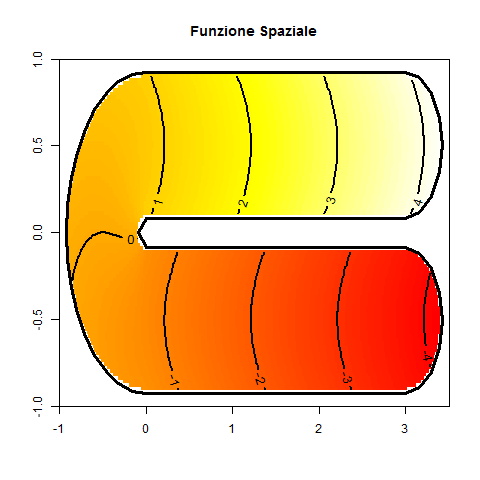
\includegraphics[width=0.46\textwidth]{Immagini/DomC_fstest.png}   
	\caption{Funzione spaziale $g(\underline p)$}
	\label{fig:domC_fstest}
\end{figure}

\section{Triangolazione e istanti temporali}
Nel dominio a forma di C non sono presenti punti spaziali definiti dalla natura del problema (come possono essere i comuni per la provincia di Venezia), quindi è stato necessario ricavarli. Sono stati generati casualmente 150 punti all'interno del rettangolo $(-1,+3.5) \times (-1,+1)$ e di questi sono stati considerati validi solo quelli che ricadevano all'interno del dominio. Non è stata usata la descrizione della frontiera presente in \textit{mgcv}, ma una versione diversa che permette di avere punti anche nella parte rettilinea del bordo.
\begin{figure}[t]
	\centering
	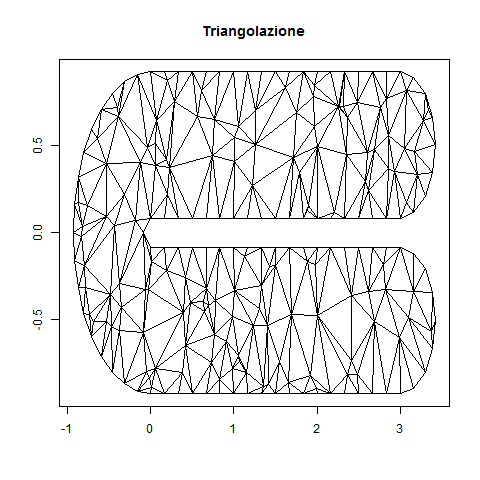
\includegraphics[width=0.46\textwidth]{Immagini/DomC_Triangolazione.png}
	\caption{Triangolazione del dominio a forma di C}
	\label{fig:domC_triang}
\end{figure}
In figura \ref{fig:domC_triang} è riportata la triangolazione ottenuta grazie al pacchetto R \textit{RTriangle}. Come basi in spazio sono stati usati gli elementi finiti lineari definiti su questa triangolazione. In tutti gli esempi che seguiranno sarà considerata questa descrizione del dominio, che è formata da 241 punti (pari anche al numero di basi spaziali $N$). Di questi 108 sono di frontiera, e i restanti 133 corrispondono agli $n$ punti sui quali saranno disponibili i dati.

Come intervallo temporale di variazione dei dati è stato scelto $[0,2\pi]$, per sfruttare la periodicità del coseno. All'interno di questo intervallo sono stati ricavati 9 istanti temporali equidistanti tra di loro, quindi uno ogni $\frac{\pi}{4}$. Si è scelto di fissare come basi in tempo le \textit{B-splines} cubiche. Il numero di basi $M$ è uguale al numero di istanti temporali a disposizione $m$, quindi 9. 

In figura \ref{fig:DomC_BSpline} sono riportate le funzioni di base B-splines che saranno usate per tutte le analisi che seguiranno.

\begin{figure}[h]
	\centering
	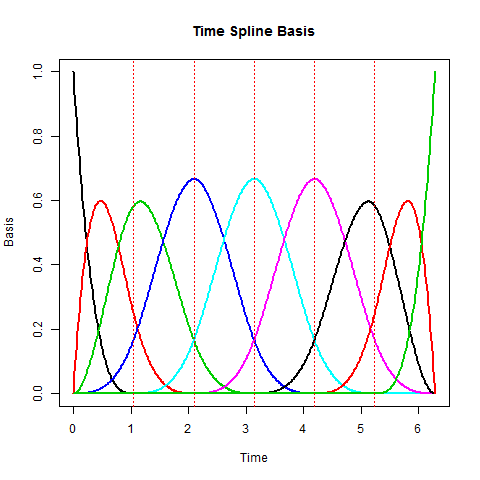
\includegraphics[width=0.55\textwidth]{Immagini/DomC_timebasis.png}   
	\caption{Basi \textit{B-splines} cubiche}
	\label{fig:DomC_BSpline}
\end{figure}

\newpage

\section{Caso senza covariate}
Nei punti e negli istanti temporali disponibili i dati sono stati ricavati dalla funzione esatta con l'aggiunta del rumore:
$$
z_{ij}=g(\underline p_{i})cos(t_j) + \varepsilon_{ij} \qquad \forall i \in 1\ldots n, \forall j \in 1\ldots m
$$
dove
$$
\varepsilon_{ij}\stackrel{\mathrm{iid}}{\sim}N(0,0.5^2) \qquad \forall i \in 1\ldots n, \forall j \in 1\ldots m \ .
$$

Per poter eseguire una analisi ottimale, come primo passo è necessario scegliere i valori per $\lambda$ ottimizzando l'indice $\mathrm{GCV}(\underline \lambda)$ come riportato in RIMANDO NECESSARIO. In queste analisi $\lambda_S$ e $\lambda_T$ sono sempre espressi in potenze di 10. Per trovare dei buoni valori per i parametri si procede per tentativi, creando due insiemi discreti di variazione per $\log_{10}\lambda_S$ e $\log_{10}\lambda_T$ e minimizzando sui $\underline \lambda$ corrispondenti al prodotto cartesiano tra di essi. Il procedimento viene iterato qualche volta (a causa dell'alto costo computazionale non è opportuno eseguire troppe iterazioni) rendendo la griglia sempre più fitta. In particolare, nel primo caso i valori sono distanziati di 1, poi (una volta che è possibile centrare gli intervalli in base al risultato precedente) di 0.25 e 0.125.

\begin{table}[htbp]
\renewcommand{\arraystretch}{1.3}
\setlength{\tabcolsep}{2mm}
\centering
	\begin{tabular}{!{\vrule width 1.2pt}c!{\vrule width 1.2pt}c!{\vrule width 1.2pt}}
	\noalign{\hrule height 1.2pt}
	Intervalli per $\log_{10}\lambda_S$ e $\log_{10}\lambda_T$& Miglior valore											\\
	\noalign{\hrule height 1.2pt}
	$\log_{10}\lambda_S \in \{-5,-4,\ldots,+1\}$ 	& \multirow{2}{*}{$\underline \lambda = (10^{0},10^{-3})$} 			\\
	\cline{1-1}
	$\log_{10}\lambda_T \in \{-5,-4,\ldots,+1\}$		& 															\\	
	\noalign{\hrule height 1.2pt}
	$\log_{10}\lambda_S \in \{-1,-0.75,\ldots,+1\}$ 	& \multirow{2}{*}{$\underline \lambda = (10^{-0.5},10^{-3.25})$} 		\\
	\cline{1-1}
	$\log_{10}\lambda_T \in \{-4,-3.75,\ldots,-2\}$	& 															\\	
	\noalign{\hrule height 1.2pt}
	$\log_{10}\lambda_S \in \{-1,-0.875,\ldots,+0\}$ 	& \multirow{2}{*}{$\underline \lambda = (10^{-0.375}, 10^{-3.25})$}	\\
	\cline{1-1}
	$\log_{10}\lambda_T \in \{-3.75,-3.625,\ldots,-2.75\}$		& 												\\	
	\noalign{\hrule height 1.2pt}
	\end{tabular}
\caption{Analisi di $\mathrm{GCV}(\underline \lambda)$}
\label{tab:DomC}
\end{table}

L'analisi è stata eseguita con $\underline \lambda = (10^{-0.375}, 10^{-3.25})$ e la stima della funzione si è rivelata molto buona.

\begin{figure}[p]
\centering
\subfigure[Funzione reale a $t=0$]
   {
	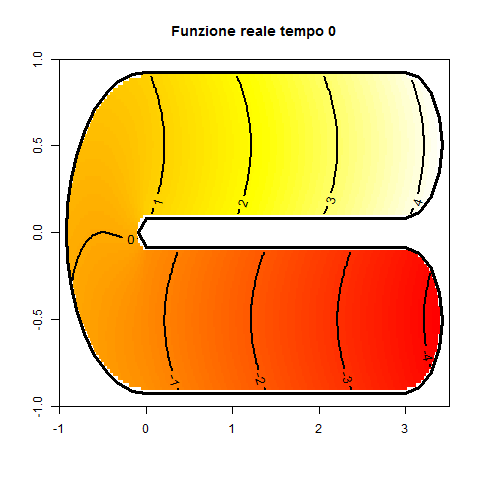
\includegraphics[width=0.46\textwidth]{Immagini/DomC_0reale.png}   
   }
\subfigure[Funzione stimata a $t=0$]
   {
	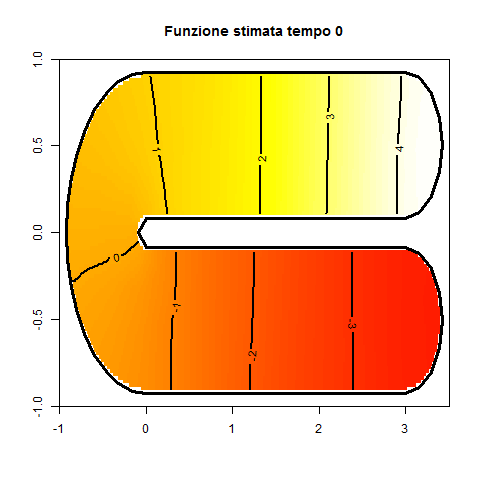
\includegraphics[width=0.46\textwidth]{Immagini/DomC_0stimata.png}
   }
\subfigure[Funzione reale a $t=\frac{\pi}{4}$]
   {
	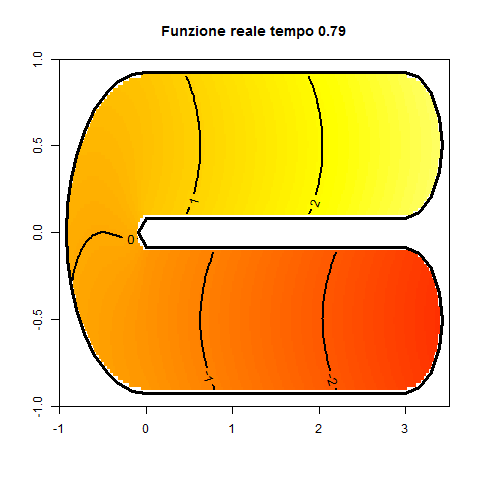
\includegraphics[width=0.46\textwidth]{Immagini/DomC_1reale.png}   
   }
\subfigure[Funzione stimata a $t=\frac{\pi}{4}$]
   {
	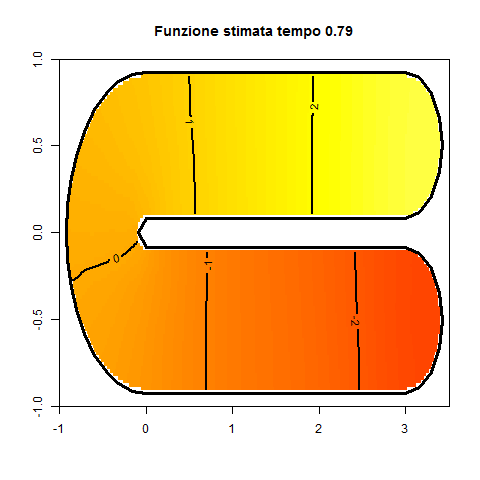
\includegraphics[width=0.46\textwidth]{Immagini/DomC_1stimata.png}
   }
\subfigure[Funzione reale a $t=\frac{\pi}{2}$]
   {
	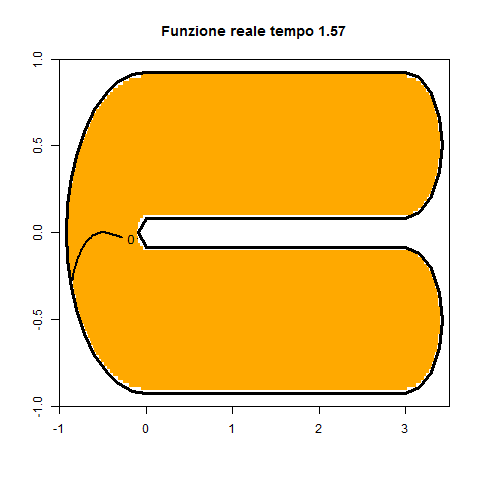
\includegraphics[width=0.46\textwidth]{Immagini/DomC_2reale.png}   
   }
\subfigure[Funzione stimata a $t=\frac{\pi}{2}$]
   {
	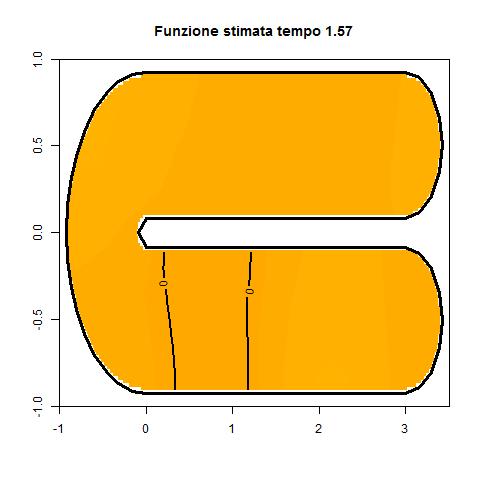
\includegraphics[width=0.46\textwidth]{Immagini/DomC_2stimata.png}
   }
\caption{Stime della funzione $f(\underline p,t)$ ad alcuni istanti di tempo, caso senza covariate}
\label{fig:DomC_ris}

\end{figure}

In figura \ref{fig:DomC_ris} sono riportati i confronti tra funzione reale e stimata nei primi istanti di tempo (la scala di colori è stata resa uniforme tra tutti i grafici). Si può notare come la funzione stimata sia effettivamente molto simile a quella reale.
\begin{figure}[h]
\centering
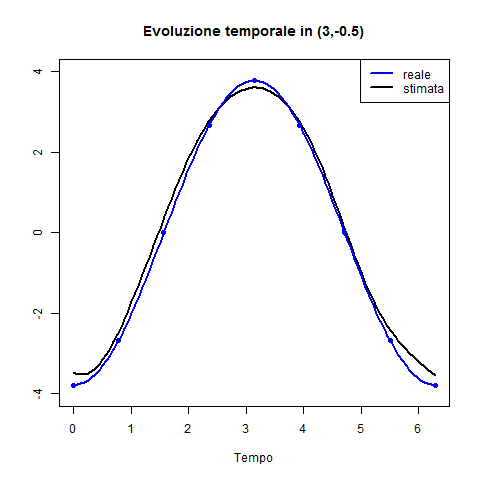
\includegraphics[width=0.46\textwidth]{Immagini/DomC_tfissato.png}   
\caption{Evoluzione temporale nel punto fissato $\underline p=(3,-0.5)$}
\label{fig:DomC_ris2}
\end{figure}

Inoltre in figura \ref{fig:DomC_ris2} si ha il confronto dell'evoluzione temporale in uno dei nodi della triangolazione. La curva reale si può è nota, ed è una cosinusoide moltiplicata per $g(3,-0.5)=-3.785398$ (funzione blu nel grafico, sono tracciati anche i dai negli istanti di tempo considerati). Si può notaLa curva stimata è molto vicina alla reale e non è una perfetta interpolazione dei dati. Questo è un ottimo risultato, poichè si è riusciti a cogliere il fenomeno temporale senza sovrastimare ed interpolare pienamente i dati (cosa che sarebbe successa con valori di $\lambda_T$ più bassi). La funzione $cos(t)$ è 



\section{Caso con covariate}
Nel problema della stima della funzione $f(\underline p,t)=g(\underline p)cos(t)$ non sono presenti covariate. Quindi per poter provare il modello in questo caso, è stato necessario generare valori da assumere come covariate in ogni punto spaziale ed istante temporale in cui si hanno le misurazioni della risposta. Quindi in definitiva i dati sono così formati:
$$
z_{ij}=g(\underline p_{i})cos(t_j) + \beta w_{ij} + \varepsilon_{ij} \qquad \forall i \in 1\ldots n, \forall j \in 1\ldots m
$$
dove covariate e rumore sono generate da due normali tra loro indipendenti:
$$
w_{ij}\stackrel{\mathrm{iid}}{\sim}N(0,1) \qquad \forall i \in 1\ldots n, \forall j \in 1\ldots m
$$
$$
\varepsilon_{ij}\stackrel{\mathrm{iid}}{\sim}N(0,0.5^2) \qquad \forall i \in 1\ldots n, \forall j \in 1\ldots m
$$
e $\beta$ è fissato a 1. Se il modello è buono, c'è da aspettarsi che la parte di funzione stimata senza covariate sia vicina a $f(\underline p,t)$ e che $\hat{\beta}$ si avvicini a 1.
 
Anche in questo caso è necessaria una analisi preliminare per fissare i valori per $\lambda$ ottimizzando l'indice $\mathrm{GCV}(\underline \lambda)$, che nel caso con covariate si differenzia dal precedente solo per la forma della \textit{smoothing matrix}. In tabella \ref{tab:DomC_covar} sono riportati i risultati ricavati secondo lo stesso approccio del caso senza covariate.

\begin{table}[htbp]
\renewcommand{\arraystretch}{1.3}
\setlength{\tabcolsep}{2mm}
\centering
	\begin{tabular}{!{\vrule width 1.2pt}c!{\vrule width 1.2pt}c!{\vrule width 1.2pt}}
	\noalign{\hrule height 1.2pt}
	Intervalli per $\log_{10}\lambda_S$ e $\log_{10}\lambda_T$& Miglior valore											\\
	\noalign{\hrule height 1.2pt}
	$\log_{10}\lambda_S \in \{-5,-4,\ldots,+1\}$ 	& \multirow{2}{*}{$\underline \lambda = (10^{0},10^{-4})$} 			\\
	\cline{1-1}
	$\log_{10}\lambda_T \in \{-5,-4,\ldots,+1\}$		& 															\\	
	\noalign{\hrule height 1.2pt}
	$\log_{10}\lambda_S \in \{-1,-0.75,\ldots,+1\}$ 	& \multirow{2}{*}{$\underline \lambda = (10^{0.25},10^{-3.75})$} 		\\
	\cline{1-1}
	$\log_{10}\lambda_T \in \{-5,-4.75,\ldots,-3\}$	& 															\\	
	\noalign{\hrule height 1.2pt}
	$\log_{10}\lambda_S \in \{-0.25,-0.125,\ldots,+0.75\}$ 	& \multirow{2}{*}{$\underline \lambda = (10^{-0.125}, 10^{-3.25})$}	\\
	\cline{1-1}
	$\log_{10}\lambda_T \in \{-4.25,-4.125,\ldots,-3.25\}$		& 												\\	
	\noalign{\hrule height 1.2pt}
	\end{tabular}
\caption{Analisi di $\mathrm{GCV}(\underline \lambda)$}
\label{tab:DomC_covar}
\end{table}

Procedendo per tentativi, si poò notare che i valori si sono rivelati molto simili al caso senza covariate riportato in \ref{tab:DomC}, lasciando pensare che la stima della funzione $f(\underline p,t)$, cioè della parte non spiegata dalla covariata, possa essere molto vicina a quella stimata nel caso senza covariate, e quindi a quella reale.

Eseguendo l'analisi con $\underline \lambda = (10^{-0.125}, 10^{-3.25})$ questa ipotesi è confermata, e si trova una buona stima della funzione. In figura \ref{fig:DomCcovar_ris} si hanno i grafici dei primi istanti di tempo (si ricorda che la funzione tracciata non contiene la parte spiegata dalle covariate, ma solo la stima di $f(\underline p,t)$). 

\newpage

\begin{figure}[h]
\centering
\subfigure[Funzione reale a $t=0$]
   {
	\includegraphics[width=0.46\textwidth]{Immagini/DomCcovar_0reale.png}   
   }
\subfigure[Funzione stimata a $t=0$]
   {
	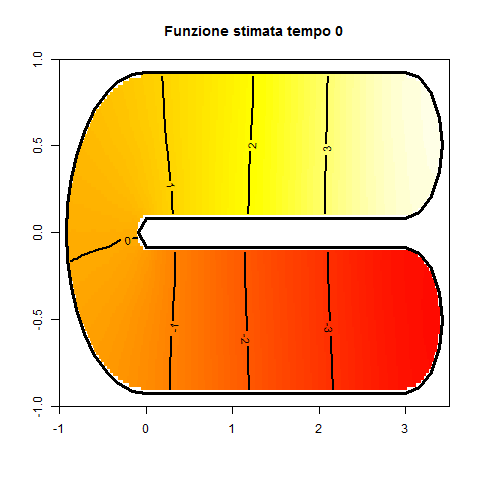
\includegraphics[width=0.46\textwidth]{Immagini/DomCcovar_0stimata.png}
   }
\subfigure[Funzione reale a $t=\frac{\pi}{4}$]
   {
	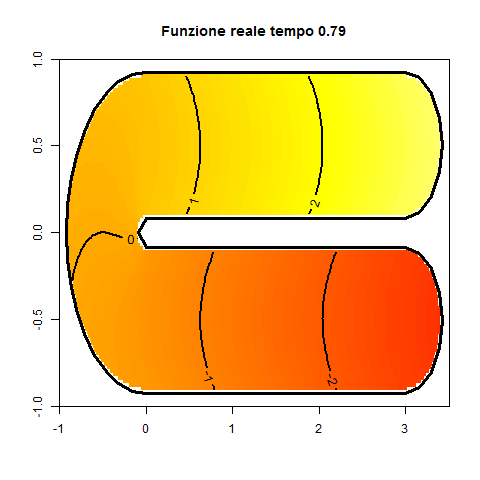
\includegraphics[width=0.46\textwidth]{Immagini/DomCcovar_1reale.png}   
   }
\subfigure[Funzione stimata a $t=\frac{\pi}{4}$]
   {
	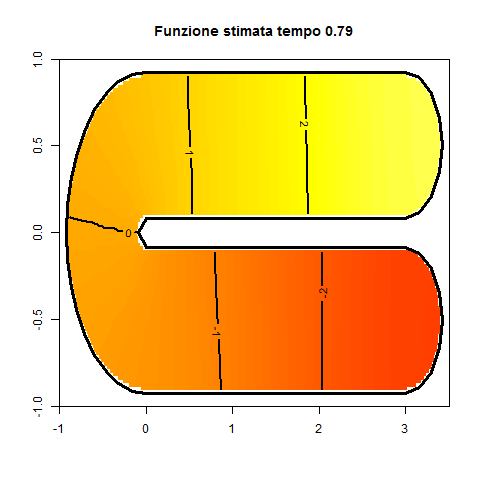
\includegraphics[width=0.46\textwidth]{Immagini/DomCcovar_1stimata.png}
   }
\subfigure[Funzione reale a $t=\frac{\pi}{2}$]
   {
	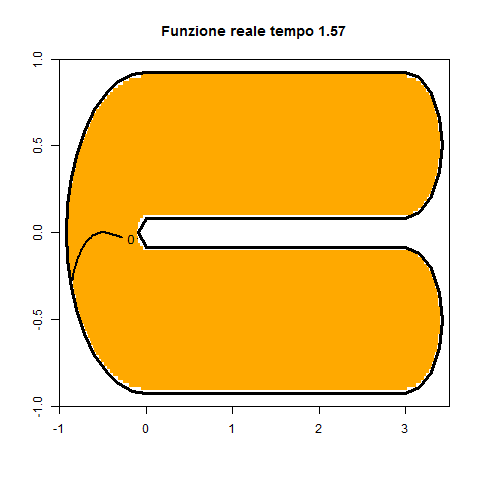
\includegraphics[width=0.46\textwidth]{Immagini/DomCcovar_2reale.png}   
   }
\subfigure[Funzione stimata a $t=\frac{\pi}{2}$]
   {
	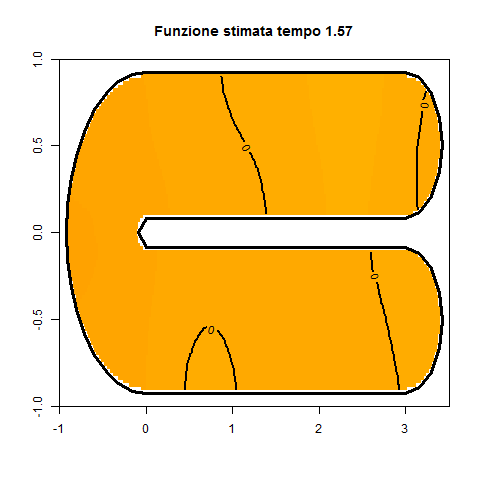
\includegraphics[width=0.46\textwidth]{Immagini/DomCcovar_2stimata.png}
   }
\caption{Stime della funzione $f(\underline p,t)$ ad alcuni istanti di tempo, caso con covariate}
\label{fig:DomCcovar_ris}
\end{figure}

Analoga al caso senza covariate è l'evoluzione temporale della funzione in uno dei nodi della triangolazione.

\begin{figure}[h]
\centering
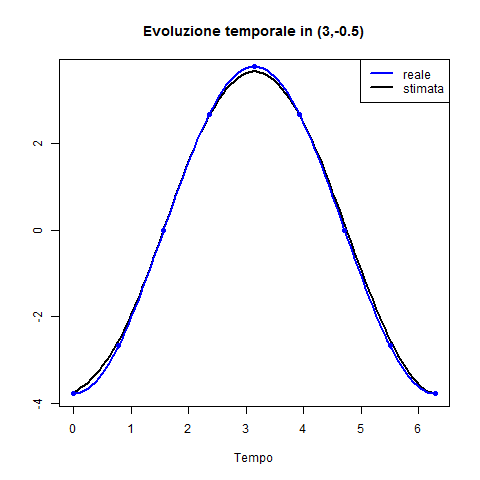
\includegraphics[width=0.46\textwidth]{Immagini/DomCcovar_tfissato.png}   
\caption{Evoluzione temporale nel punto fissato $\underline p=(3,-0.5)$}
\label{fig:DomCcovar_ris2}
\end{figure}

Dai grafici precedenti si può trarre come conclusione che la stima della parte funzionale della risposta sia effettivamente una buona approssimazione della reale. Tuttavia occorre verificare anche che il contributo delle covariate sia ben riconosciuto dal modello, e per questo basta controllare il valore stimato di $\beta$. Si ha:
$$
\hat{\beta} \approx 1.005 \ ,
$$
valore vicinissimo al reale.


GRAFICI DEI RESIDUI???



\end{document}